\begin{tblr}{|Q[c,m]|l|l|l|}
	\SetHline[1]{1-6}{blue5,1pt}
	\SetHline[2]{1-6}{azure5,1pt}
	\hline
	\SetCell[c=4]{c} Elemento 1 \\
	\hline
	Tentativas & Medição (cm) & Medição (m) $\pm 0.003$ (m) &  Tempo de Reação  (s)\\ \hline	 
	1 & 10.7 &  0.107 & 1.48E-01 \\\hline
	2 & 17 & 0.170 & 1.86E-01  \\\hline
	3 & 12.3 &  0.123  & 1.58E-01  \\\hline
	4 & 9.8 &   0.098 & 1.41E-01 \\\hline
	5 & 14 &    0.140  & 1.69E-01  \\\hline
	6 & 9.8 &    0.098 & 1.41E-01\\\hline
	7 & 11.1 &  0.111  & 1.50E-01 \\\hline
	8 & 10.8 &  0.108 & 1.48E-01 \\\hline
	9 & 14   &  0.140  & 1.69E-01 \\\hline
	10 & 14.9 & 0.149 & 1.74E-01 \\\hline
	11 & 23.2 & 0.232 & 2.18E-01  \\\hline
	12 & 10.2 & 0.102 & 1.44E-01 \\\hline
	13 & 11.8 & 0.118  & 1.55E-01\\\hline
	14 & 13.4 & 0.134 & 1.65E-01 \\\hline
	15 & 10.1 & 0.101 & 1.44E-01 \\\hline
	16 & 15.5 & 0.155 & 1.78E-01 \\\hline
	17 & 20.4 & 0.204 & 2.04E-01 \\\hline
	18 & 17.9 & 0.179 & 1.91E-01 \\\hline
	19 & 11.7 & 0.116 & 1.55E-01  \\\hline
	20 & 11.3 & 0.113 & 1.52E-01 \\\hline
	\hline
	\SetHline[1]{1-4}{teal5,1pt}
	\SetHline[2]{1-4}{green5,1pt}
\end{tblr}

\begin{tblr}{|llll|}
	Média & 1.65E-01 (s) & Desvio Padrão & $\pm$ 2.11E-02 (s) \\
	\SetHline[1]{1-6}{teal5,1pt}
	\SetHline[2]{1-6}{green5,1pt}
\end{tblr}


\begin{tblr}{|Q[c,m]|l|l|l|}
	\SetHline[1]{1-6}{blue5,1pt}
	\SetHline[2]{1-6}{azure5,1pt}
	\hline
	\SetCell[c=4]{c} Elemento 2 \\
	\hline
	Tentativas & Medição (cm) & Medição (m) $\pm 0.002$ (m) &  Tempo de Reação (s)\\ \hline
	1 & 9.8  & 0.098 & 1.41E-01 \\\hline
	2 & 13.3  & 0.133 &  1.65E-01 \\\hline
	3 & 19  & 0.190 & 1.97E-01\\\hline	
	4 & 15.5  &  0.155 & 1.78E-01 \\\hline
	5 & 13  & 0.130 & 1.63E-01\\\hline
	6 &  12.5 & 0.125 & 1.60E-01\\\hline
	7 &  15.7 & 0.157 & 1.79E-01\\\hline
	8 &  14 &  0.140 & 1.69E-01\\\hline
	9 &  17 & 0.170 & 1.86E-01 \\\hline
	10 & 7.5 & 0.750 & 1.24E-01\\\hline
	11 & 14.5 & 0.145 & 1.72E-01 \\\hline
	12 & 14 & 0.140 & 1.69E-01\\\hline
	13 & 9.7 &  0.097 & 1.41E-01\\\hline
	14 & 17 & 0.170 & 1.86E-01 \\\hline
	15 & 14 & 0.140 & 1.69E-01 \\\hline
	16 & 11.5 & 0.115 & 1.53E-01 \\\hline
	17 & 11 & 0.110 & 1.50E-01 \\\hline
	18 & 11.5 & 0.115 & 1.53E-01\\\hline
	19 & 14 & 0.140 & 1.69E-01 \\\hline
	20 &  13.7& 0.137 & 1.67E-01 \\\hline
	\hline
	\SetHline[1]{1-4}{teal5,1pt}
	\SetHline[2]{1-4}{green5,1pt}
	\hline
\end{tblr}

\begin{tblr}{|llll|}
	Média & 1.70E-02(s) & Desvio Padrão & $\pm$ 1.70E-02 (s) \\
	\SetHline[1]{1-6}{teal5,1pt}
	\SetHline[2]{1-6}{green5,1pt}
\end{tblr}

\begin{tblr}{|Q[c,m]|l|l|l|}
	\SetHline[1]{1-6}{blue5,1pt}
	\SetHline[2]{1-6}{azure5,1pt}
	\hline
	\SetCell[c=4]{c} Elemento 3 \\
	\hline
	Tentativas & Medição (cm) & Medição (m) $\pm 0.006$ (m) &  Tempo de Reação (s)\\ \hline
	1 & 20  & 0.200 & 2.02E-01 \\\hline
	2 & 9  & 0.090 &  1.36E-01 \\\hline
	3 & 15  & 0.150 & 1.75E-01\\\hline	
	4 & 7  &  0.070 & 1.20E-01 \\\hline
	5 & 5  & 0.050 & 1.01E-01\\\hline
	6 &  20 & 0.200 & 2.02E-01\\\hline
	7 &  15 & 0.150 & 1.75E-01\\\hline
	8 &  20 &  0.200 & 2.02E-01\\\hline
	9 &  20 & 0.200 & 2.02E-01 \\\hline
	10 & 11 & 0.110 & 1.50E-01\\\hline
	11 & 17 & 0.170 & 1.86E-01 \\\hline
	12 & 11 & 0.110 & 1.50E-01\\\hline
	13 & 17 &  0.170 & 1.86E-01\\\hline
	14 & 12 & 0.120 & 1.56E-01 \\\hline
	15 & 6 & 0.060 & 1.11E-01 \\\hline
	16 & 12 & 0.120 & 1.56E-01 \\\hline
	17 & 6 & 0.060 & 1.11E-01 \\\hline
	18 & 18 & 0.180 & 1.92E-01\\\hline
	19 & 17 & 0.170 & 1.86E-01 \\\hline
	20 & 16& 0.160 & 1.81E-01 \\\hline
	\hline
	\SetHline[1]{1-4}{teal5,1pt}
	\SetHline[2]{1-4}{green5,1pt}
	\hline
\end{tblr}

\begin{tblr}{|llll|}
	Média & 1.64E-01(s) & Desvio Padrão & $\pm$ 3.36E-02(s) \\
	\SetHline[1]{1-6}{teal5,1pt}
	\SetHline[2]{1-6}{green5,1pt}
\end{tblr}

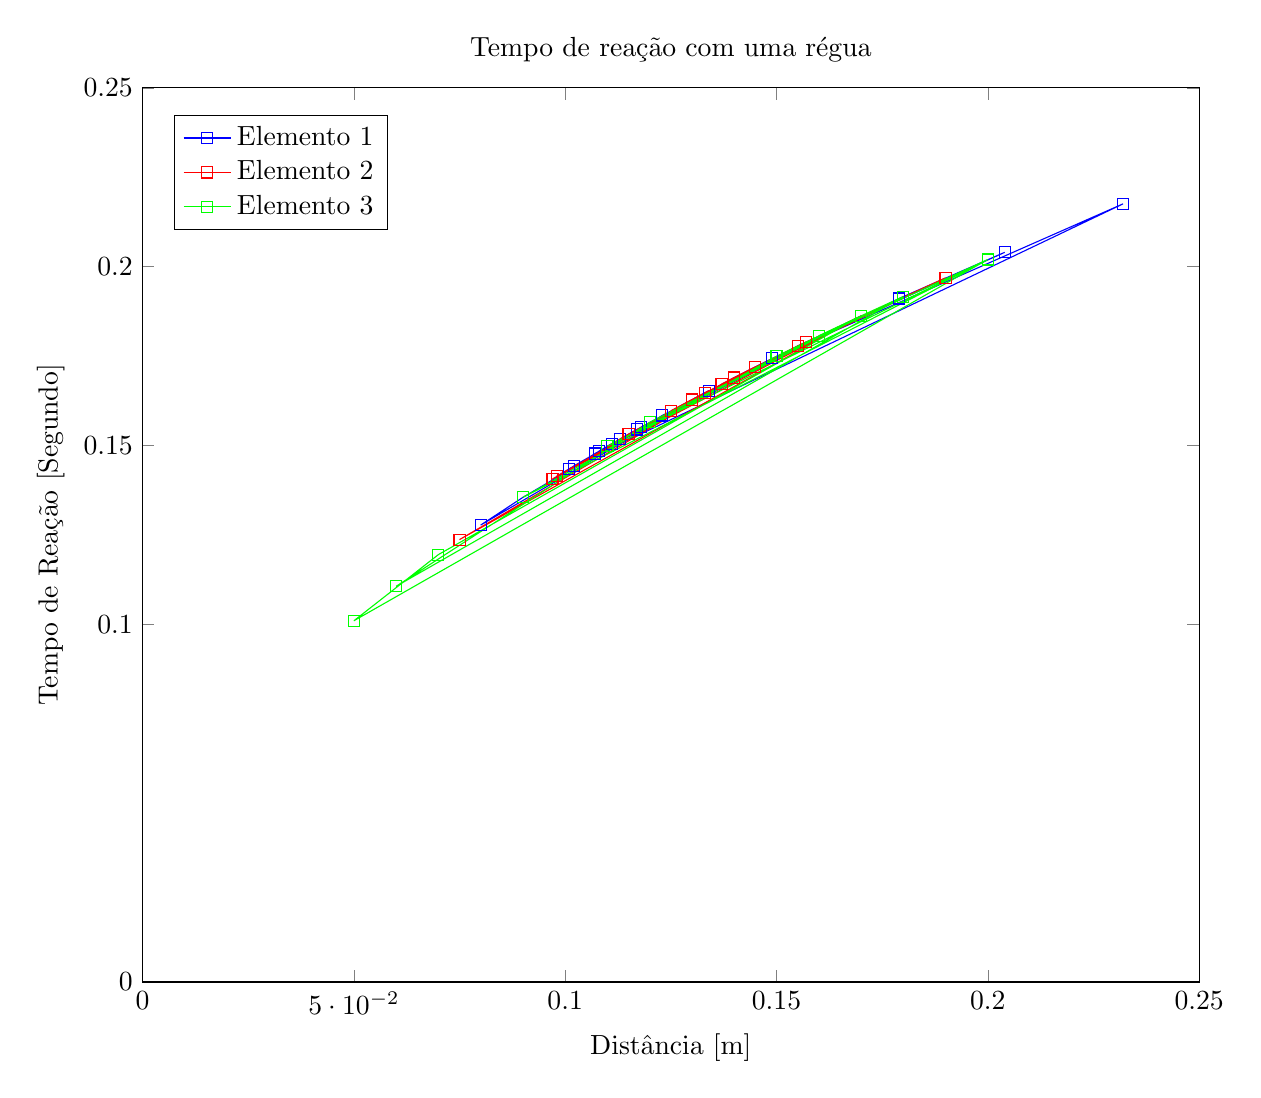
\begin{tikzpicture}
	\pgfplotsset{width=15cm,compat=newest}
	\begin{axis}[
		title={Tempo de reação com uma régua},
		xlabel={Distância [m]},
		ylabel={Tempo de Reação [Segundo]},
		xmin=0, xmax=0.25,
		ymin=0, ymax=0.25,
		xtick={0,0.05,0.10,0.15,0.20,0.25},
		ytick={0,0.10,0.15,0.20,0.25},
		legend pos=north west,
		%ymajorgrids=true,
		grid style=dashed,
		]	
		\addplot[
		color=blue,
		mark=square,
		]
		coordinates {
	(0.107, 0.14775750108440802)
	(0.17, 0.18624392235057782)
	(0.12300000000000001, 0.15842007131712585)
	(0.09, 0.13551235834954697)
	(0.08, 0.1277622766980615)
	(0.14, 0.1690136055392466)
	(0.098, 0.14140692769508584)
	(0.111, 0.15049398358094732)
	(0.10800000000000001, 0.14844635097754083)
	(0.14, 0.1690136055392466)
	(0.149, 0.17436157484928166)
	(0.23199999999999998, 0.21757131728816848)
	(0.102, 0.14426392191922704)
	(0.11800000000000001, 0.1551667459120389)
	(0.134, 0.1653522267958483)
	(0.100999999999999, 0.14355500400779636)
	(0.155, 0.17783756277837381)
	(0.204, 0.2040199949393041)
	(0.179, 0.191110330801539)
	(0.11699999999999999, 0.1545078607873814)
	(0.113, 0.15184373242824098)};
		\legend{Elemento 1}
		
		\addplot[
		color=red,
		mark=square,
		]
		coordinates {
			(0.098, 0.14140692769508584)
			(0.133, 0.16473408546657017)
			(0.19, 0.19689489188218182)
			(0.155, 0.17783756277837381)
			(0.13, 0.16286558549611407)
			(0.125, 0.15970284587257685)
			(0.157, 0.17898122448633783)
			(0.14, 0.1690136055392466)
			(0.17, 0.18624392235057782)
			(0.075, 0.12370529248128402)
			(0.145, 0.17200522903844537)
			(0.14, 0.1690136055392466)
			(0.09699999999999999, 0.14068361385863257)
			(0.17, 0.18624392235057782)
			(0.14, 0.1690136055392466)
			(0.115, 0.15318158851969135)
			(0.11, 0.14981454903387734)
			(0.115, 0.15318158851969135)
			(0.14, 0.1690136055392466)
			(0.13699999999999998, 0.16719293909092225)
		};
		\addlegendentry{Elemento 2}
		
		\addplot[
		color=green,
		mark=square,
		]
		coordinates {
			(0.2, 0.2020098967072655)
			(0.09, 0.13551235834954697)
			(0.15, 0.17494570236436233)
			(0.17, 0.18624392235057782)
			(0.07, 0.1195106665895895)
			(0.05, 0.10100494835363275)
			(0.2, 0.2020098967072655)
			(0.15, 0.17494570236436233)
			(0.2, 0.2020098967072655)
			(0.2, 0.2020098967072655)
			(0.11, 0.14981454903387734)
			(0.17, 0.18624392235057782)
			(0.11, 0.14981454903387734)
			(0.17, 0.18624392235057782)
			(0.12, 0.15647619314326394)
			(0.06, 0.11064537726585788)
			(0.12, 0.15647619314326394)
			(0.06, 0.11064537726585788)
			(0.18, 0.19164341504709223)
			(0.17, 0.18624392235057782)
			(0.16, 0.18068314446606262)
		};
		\addlegendentry{Elemento 3}
		
	\end{axis}
\end{tikzpicture}


